% Created by tikzDevice version 0.7.0 on 2015-04-27 12:39:19
% !TEX encoding = UTF-8 Unicode
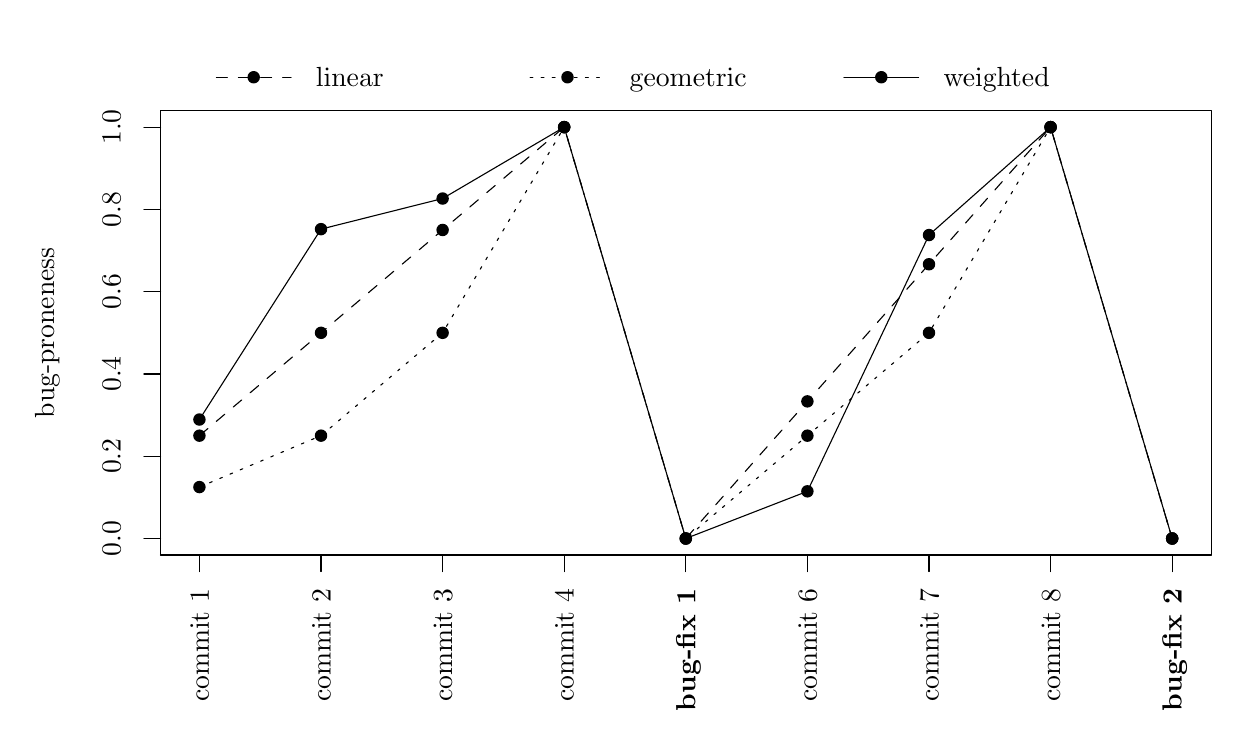
\begin{tikzpicture}[x=1pt,y=1pt]
\definecolor[named]{fillColor}{rgb}{1.00,1.00,1.00}
\path[use as bounding box,fill=fillColor,fill opacity=0.00] (0,0) rectangle (433.62,252.94);
\begin{scope}
\path[clip] ( 48.00, 62.40) rectangle (427.62,222.94);
\definecolor[named]{drawColor}{rgb}{0.00,0.00,0.00}

\path[draw=drawColor,line width= 0.4pt,dash pattern=on 4pt off 4pt ,line join=round,line cap=round] ( 62.06,105.51) --
	(106.00,142.67) --
	(149.94,179.84) --
	(193.87,217.00) --
	(237.81, 68.35) --
	(281.75,117.90) --
	(325.69,167.45) --
	(369.62,217.00) --
	(413.56, 68.35);
\end{scope}
\begin{scope}
\path[clip] (  0.00,  0.00) rectangle (433.62,252.94);
\definecolor[named]{drawColor}{rgb}{0.00,0.00,0.00}

\path[draw=drawColor,line width= 0.4pt,line join=round,line cap=round] ( 48.00, 68.35) -- ( 48.00,217.00);

\path[draw=drawColor,line width= 0.4pt,line join=round,line cap=round] ( 48.00, 68.35) -- ( 42.00, 68.35);

\path[draw=drawColor,line width= 0.4pt,line join=round,line cap=round] ( 48.00, 98.08) -- ( 42.00, 98.08);

\path[draw=drawColor,line width= 0.4pt,line join=round,line cap=round] ( 48.00,127.81) -- ( 42.00,127.81);

\path[draw=drawColor,line width= 0.4pt,line join=round,line cap=round] ( 48.00,157.54) -- ( 42.00,157.54);

\path[draw=drawColor,line width= 0.4pt,line join=round,line cap=round] ( 48.00,187.27) -- ( 42.00,187.27);

\path[draw=drawColor,line width= 0.4pt,line join=round,line cap=round] ( 48.00,217.00) -- ( 42.00,217.00);

\node[text=drawColor,rotate= 90.00,anchor=base,inner sep=0pt, outer sep=0pt, scale=  1.00] at ( 33.60, 68.35) {0.0};

\node[text=drawColor,rotate= 90.00,anchor=base,inner sep=0pt, outer sep=0pt, scale=  1.00] at ( 33.60, 98.08) {0.2};

\node[text=drawColor,rotate= 90.00,anchor=base,inner sep=0pt, outer sep=0pt, scale=  1.00] at ( 33.60,127.81) {0.4};

\node[text=drawColor,rotate= 90.00,anchor=base,inner sep=0pt, outer sep=0pt, scale=  1.00] at ( 33.60,157.54) {0.6};

\node[text=drawColor,rotate= 90.00,anchor=base,inner sep=0pt, outer sep=0pt, scale=  1.00] at ( 33.60,187.27) {0.8};

\node[text=drawColor,rotate= 90.00,anchor=base,inner sep=0pt, outer sep=0pt, scale=  1.00] at ( 33.60,217.00) {1.0};

\path[draw=drawColor,line width= 0.4pt,line join=round,line cap=round] ( 48.00, 62.40) --
	(427.62, 62.40) --
	(427.62,222.94) --
	( 48.00,222.94) --
	( 48.00, 62.40);
\end{scope}
\begin{scope}
\path[clip] (  0.00,  0.00) rectangle (433.62,252.94);
\definecolor[named]{drawColor}{rgb}{0.00,0.00,0.00}

\node[text=drawColor,rotate= 90.00,anchor=base,inner sep=0pt, outer sep=0pt, scale=  1.00] at (  9.60,142.67) {bug-proneness};
\end{scope}
\begin{scope}
\path[clip] ( 48.00, 62.40) rectangle (427.62,222.94);
\definecolor[named]{fillColor}{rgb}{0.00,0.00,0.00}

\path[fill=fillColor] ( 62.06,105.51) circle (  2.25);

\path[fill=fillColor] (106.00,142.67) circle (  2.25);

\path[fill=fillColor] (149.94,179.84) circle (  2.25);

\path[fill=fillColor] (193.87,217.00) circle (  2.25);

\path[fill=fillColor] (237.81, 68.35) circle (  2.25);

\path[fill=fillColor] (281.75,117.90) circle (  2.25);

\path[fill=fillColor] (325.69,167.45) circle (  2.25);

\path[fill=fillColor] (369.62,217.00) circle (  2.25);

\path[fill=fillColor] (413.56, 68.35) circle (  2.25);
\definecolor[named]{drawColor}{rgb}{0.00,0.00,0.00}

\path[draw=drawColor,line width= 0.4pt,dash pattern=on 1pt off 3pt ,line join=round,line cap=round] ( 62.06, 86.93) --
	(106.00,105.51) --
	(149.94,142.67) --
	(193.87,217.00) --
	(237.81, 68.35) --
	(281.75,105.51) --
	(325.69,142.67) --
	(369.62,217.00) --
	(413.56, 68.35);

\path[fill=fillColor] ( 62.06, 86.93) circle (  2.25);

\path[fill=fillColor] (106.00,105.51) circle (  2.25);

\path[fill=fillColor] (149.94,142.67) circle (  2.25);

\path[fill=fillColor] (193.87,217.00) circle (  2.25);

\path[fill=fillColor] (237.81, 68.35) circle (  2.25);

\path[fill=fillColor] (281.75,105.51) circle (  2.25);

\path[fill=fillColor] (325.69,142.67) circle (  2.25);

\path[fill=fillColor] (369.62,217.00) circle (  2.25);

\path[fill=fillColor] (413.56, 68.35) circle (  2.25);

\path[draw=drawColor,line width= 0.4pt,line join=round,line cap=round] ( 62.06,111.34) --
	(106.00,180.14) --
	(149.94,191.20) --
	(193.87,217.00) --
	(237.81, 68.35) --
	(281.75, 85.40) --
	(325.69,178.01) --
	(369.62,217.00) --
	(413.56, 68.35);

\path[fill=fillColor] ( 62.06,111.34) circle (  2.25);

\path[fill=fillColor] (106.00,180.14) circle (  2.25);

\path[fill=fillColor] (149.94,191.20) circle (  2.25);

\path[fill=fillColor] (193.87,217.00) circle (  2.25);

\path[fill=fillColor] (237.81, 68.35) circle (  2.25);

\path[fill=fillColor] (281.75, 85.40) circle (  2.25);

\path[fill=fillColor] (325.69,178.01) circle (  2.25);

\path[fill=fillColor] (369.62,217.00) circle (  2.25);

\path[fill=fillColor] (413.56, 68.35) circle (  2.25);
\end{scope}
\begin{scope}
\path[clip] (  0.00,  0.00) rectangle (433.62,252.94);
\definecolor[named]{drawColor}{rgb}{0.00,0.00,0.00}

\path[draw=drawColor,line width= 0.4pt,line join=round,line cap=round] ( 62.06, 62.40) -- (413.56, 62.40);

\path[draw=drawColor,line width= 0.4pt,line join=round,line cap=round] ( 62.06, 62.40) -- ( 62.06, 56.40);

\path[draw=drawColor,line width= 0.4pt,line join=round,line cap=round] (106.00, 62.40) -- (106.00, 56.40);

\path[draw=drawColor,line width= 0.4pt,line join=round,line cap=round] (149.94, 62.40) -- (149.94, 56.40);

\path[draw=drawColor,line width= 0.4pt,line join=round,line cap=round] (193.87, 62.40) -- (193.87, 56.40);

\path[draw=drawColor,line width= 0.4pt,line join=round,line cap=round] (237.81, 62.40) -- (237.81, 56.40);

\path[draw=drawColor,line width= 0.4pt,line join=round,line cap=round] (281.75, 62.40) -- (281.75, 56.40);

\path[draw=drawColor,line width= 0.4pt,line join=round,line cap=round] (325.69, 62.40) -- (325.69, 56.40);

\path[draw=drawColor,line width= 0.4pt,line join=round,line cap=round] (369.62, 62.40) -- (369.62, 56.40);

\path[draw=drawColor,line width= 0.4pt,line join=round,line cap=round] (413.56, 62.40) -- (413.56, 56.40);

\node[text=drawColor,rotate= 90.00,anchor=base east,inner sep=0pt, outer sep=0pt, scale=  1.00] at ( 65.50, 50.40) {commit 1};

\node[text=drawColor,rotate= 90.00,anchor=base east,inner sep=0pt, outer sep=0pt, scale=  1.00] at (109.44, 50.40) {commit 2};

\node[text=drawColor,rotate= 90.00,anchor=base east,inner sep=0pt, outer sep=0pt, scale=  1.00] at (153.38, 50.40) {commit 3};

\node[text=drawColor,rotate= 90.00,anchor=base east,inner sep=0pt, outer sep=0pt, scale=  1.00] at (197.32, 50.40) {commit 4};

\node[text=drawColor,rotate= 90.00,anchor=base east,inner sep=0pt, outer sep=0pt, scale=  1.00] at (241.25, 50.40) {\textbf{bug-fix 1}};

\node[text=drawColor,rotate= 90.00,anchor=base east,inner sep=0pt, outer sep=0pt, scale=  1.00] at (285.19, 50.40) {commit 6};

\node[text=drawColor,rotate= 90.00,anchor=base east,inner sep=0pt, outer sep=0pt, scale=  1.00] at (329.13, 50.40) {commit 7};

\node[text=drawColor,rotate= 90.00,anchor=base east,inner sep=0pt, outer sep=0pt, scale=  1.00] at (373.07, 50.40) {commit 8};

\node[text=drawColor,rotate= 90.00,anchor=base east,inner sep=0pt, outer sep=0pt, scale=  1.00] at (417.00, 50.40) {\textbf{bug-fix 2}};
\end{scope}
\begin{scope}
\path[clip] (  0.00,  0.00) rectangle (433.62,252.94);
\definecolor[named]{drawColor}{rgb}{0.00,0.00,0.00}

\path[draw=drawColor,line width= 0.4pt,dash pattern=on 4pt off 4pt ,line join=round,line cap=round] ( 68.17,235.03) -- ( 95.17,235.03);

\path[draw=drawColor,line width= 0.4pt,dash pattern=on 1pt off 3pt ,line join=round,line cap=round] (181.56,235.03) -- (208.56,235.03);

\path[draw=drawColor,line width= 0.4pt,line join=round,line cap=round] (294.96,235.03) -- (321.96,235.03);
\definecolor[named]{fillColor}{rgb}{0.00,0.00,0.00}

\path[fill=fillColor] ( 81.67,235.03) circle (  2.25);

\path[fill=fillColor] (195.06,235.03) circle (  2.25);

\path[fill=fillColor] (308.46,235.03) circle (  2.25);

\node[text=drawColor,anchor=base west,inner sep=0pt, outer sep=0pt, scale=  1.00] at (104.17,231.58) {linear};

\node[text=drawColor,anchor=base west,inner sep=0pt, outer sep=0pt, scale=  1.00] at (217.56,231.58) {geometric};

\node[text=drawColor,anchor=base west,inner sep=0pt, outer sep=0pt, scale=  1.00] at (330.96,231.58) {weighted};
\end{scope}
\end{tikzpicture}
